\section{Methodology}

\subsection{Minimum Spanning Tree}
\label{sec:mst}
% Johann

For the further report, it is assumed, that the reader is familiar with the concept of
an \ac{MST}. For the unfamiliar reader, a look at \cite[pp. 585ff.]{cormen_introduction_2022}
is suggested.

For this project, the \ac{MST}s are being calculated using
Prim's Algorithm.

\subsubsection{Prim's Algorithm}

Prim's Algorithm is a well-known algorithm used for 
finding \ac{MST}s in graphs.
The following Definition of the algorithm is adapted from
\cite[p. 596]{cormen_introduction_2022}.

\begin{minted}[mathescape=true, escapeinside=||]{text}
// G: a graph
// G.V: List of all vertices in G
// G.Adj: G.Adj[u] is a List of all vertices that are adjacent to u
// w: w(u,v) == weight of the edge between u and v
// r: root / starting vertex for the algorithm
MST-PRIM(G, w, r)
  for each vertex u in G.V
    u.key = |$\infty$|
    u.pi = NIL
  r.key = 0
  Q = PriorityQueue::empty()
  for each vertex u in G.V
    Q.insert(u)
  while not Q.is_empty()
    u = Q.extract_min() // add u to the tree
    for each vertex v in G.Adj[u] // update keys of u's non-tree neighbors
      if v in Q and w(u, v) < v.key
        v.pi = u
        v.key = w(u,v)
        Q.update_key(v, w(u,v))
\end{minted}

The implementation of the PriorityQueue can be done with different
data structures.
A na\"ive way is to use vectors with linear search,
where a single \texttt{extract\_min} Operation takes linear time.
There are more sophisticated implementations using
binary or Fibonacci heaps, that improve the asymptotic
time demand of Prim's algorithm.
However, when testing the different implementations on
TSPLIB instances \cite{reinelt_tsplib_nodate}, it becomes clear that the
graph sizes are too small to benefit from asymptotic improvements,
and the simple linear search approach is the fastest.
This is likely a consequence of the higher locality and simplicity
of the code, giving rise to better compile-time optimizations,
better branch prediction, and many other optimizations.

It is possible to parallelize linear search on a vector.
However, due to the graphs for a \ac{TSP} instance being relatively small
in terms of nodes, there was very little benefit in using parallelization
for the tested use cases.
Even more so, the overhead created by the parallelization framework oftentimes
outweighed the benefits of parallel computation.
Nevertheless, a parallel implementation
for shared memory is provided,
relying on the rayon \texttt{ParallelIterator} implementation
to handle the exact details.
Although an implementation using \ac{MPI} is possible,
the results from the rayon benchmarks suggest that there
is little benefit in implementing it for this use case,
as can be seen in section \ref{sec:mst_bench}.

\subsection{Exact and Approximate Solving}
Since it is known to be \acs{NP}\footnote{\acf{NP}} complete, the \ac{TSP} is very hard to solve. While the na\"ive implementation is $\Theta(n!)$ time and $\Theta(n^2)$ space\footnote{Which is the minimum to hold the graph itself.}, even highly optimized, dynamic programming-based algorithms such as the well-known Held-Karp algorithm \cite{held_dynamic_1962} still require $\Theta(2^n n^2)$ time with $\Theta(n 2^n)$ space complexity for caching; $n$ being the number of nodes. This implies that, for large graphs, the computation is too time-expensive. More importantly, a sub-exponential algorithm is very unlikely to be found in the future, as it would implicitly prove that $P=NP$.

With such a hard problem, which, as mentioned in the introduction, has many applications in real life, the need for sub-exponential approximation algorithms becomes obvious. Walky supports both exact solving and finding approximate solutions. In this chapter, the focus will first be on exact solving, starting with the na\"ive $\Theta(n!)$ algorithm which will then be optimized and parallelized using traditional performance optimization methods. After that, two different approximation algorithms will be covered. Lastly, two more algorithms for computing the lower bound will be presented.

\subsection{Exact Solving}
This section will focus on the exact solving. Starting with the most na\"ive, sequential implementation, this report will iteratively optimize the runtime using traditional performance engineering. Note that many of the ideas are inspired by the related \ac{TSP} lecture from the MIT 6.172 course ``Performance Engineering of Software Systems'' \cite{bentley_lecture_2018}.

\subsubsection{Sequential Algorithms}
This section will use pseudo-code whenever possible to simplify the algorithmic concepts explained.

\paragraph{Version 0: Na\"ive implementation:}

For a $n$-vertex graph, with vertices numbered $1,\dots,n$, a tour can be described as an $n$-dimensional vector where each number $[1,n]$ can occur only once. Thus, testing all possible tours for the shortest one is equivalent to trying out all permutations of the vector $(1,\dots,n)$. In pseudocode:

\begin{figure}[H]
\begin{minted}[mathescape=true, escapeinside=||]{python}
def tsp_solver(G):
  path = [1..n]
  least_cost = inf
  while (has_next_permutation(path)):
    current_cost = evaluate(path)
    if (current_cost < least_cost):
      least_cost = current_cost
    path = next_permutation(path)
  return least_cost
\end{minted}
\caption{Na\"ive implementation of a \ac{TSP} solver in pseudocode.}
\end{figure}

Since there are $(\prod_{i=1}^n i) = n!$ possible permutations, this algorithm has a time complexity of $\Theta(n!)$. For enumeration, Nayuiki's iterative next lexicographical permutation algorithm was used \cite{nayuki_next_2018}.

\paragraph{Version 1: Fix the first element:}

The \ac{TSP} is defined as the shortest path traveling through all cities \emph{and returning to the origin}. Since a tour is cyclic, the vectors $(1,2,3)$, $(3,1,2)$, and $(2,3,1)$ all represent the same underlying tour. Thus, one can reduce the time complexity to $\Theta((n-1)!)$ by fixing the first element.

\paragraph{Version 2 and 3: Prune if the subpath is non-optimal:}

Version 2 caches the subpaths, reducing the amount of additions required to compute the tour cost.\\

Starting with version 3, the next algorithm iterations will heavily rely on decision tree pruning. This is best explained by an example:

\begin{example}{Pruning}
Let $G$ be an $n$-dimensional, fully connected, undirected symmetric graph for which the \ac{TSP} is being solved. W.l.o.g let $35$ be the current optimal known cost.

Let us further assume that the path $(4,5,6)$ has cost $36$. Since edge costs can't be negative, this means that all paths with the prefix $(4,5,6)$ can't be better than the already known optimum, thus they can be \emph{pruned}.
\end{example}

Hence, instead of iterating over all possible solutions as a whole, the partial sums of the subtours will be cached using \textbf{recursive enumeration}:

\begin{figure}[H]
\centering
\begin{subfigure}[b]{0.45\textwidth}
\begin{minted}[mathescape=true, escapeinside=||]{python}
def rec_enum(xs, n):
  """Recursively enumerate xs"""
  if len(xs) == n: # Full path
    print(xs)
  for i in range(n):
    if i not in xs:
      rec_enum(xs + [i], n)
\end{minted}
\caption{Pseudocode of recursive enumeration}
\end{subfigure}
\hfill
\begin{subfigure}[b]{0.45\textwidth}
\centering
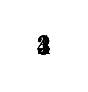
\begin{tikzpicture}[every tree node/.style={draw,circle}]
    \Tree [.\node{1};
            [.\node{2};
                [.\node{3};
                    [.\node{4}; ]
                ]
                [.\node{4};
                    [.\node{3}; ]
                ]
            ]
            [.\node{3};
                [.\node{2};
                    [.\node{4}; ]
                ]
                [.\node{4};
                    [.\node{2}; ]
                ]
            ]
            [.\node{4};
                [.\node{2};
                    [.\node{3}; ]
                ]
                [.\node{3};
                    [.\node{2}; ]
                ]
            ]
        ]
\end{tikzpicture}
\caption{All permutations of $(1,2,3,4)$, with $1$ fixed as the first element, visualized as a decision tree.}
\end{subfigure}
\caption{A pseudocode and visual representation of a recursive enumeration}
\end{figure}

Therefore, version 3 uses recursive enumeration for the tour generation, computing the sub-tour cost on each level, and pruning whenever the partial sum is bigger than the previously known optimum by not recursing deeper.

Analogous to this approach, the next versions will use pruning extensively to achieve better performance by reducing the number of permutations to compute the cost for.

\paragraph{Version 4: Prune using \ac{NN} Metric:}

In version 3, the subgraph was pruned iff it already costs more than the previously known minimum. To prune more aggressively, now a subgraph will be pruned iff its cost plus a lower bound on the remaining vertices is bigger than the current minimum. A graph qualifies as a lower bound if its cumulative cost is below the sum of the costs of the vertices added to the \ac{TSP} solution;

Here, the \acl{NN} lower bound will be used\footnote{Not to be confused with the \acl{NN} algorithm used for approximating a solution.}. The \ac{NN} graph will be computed by connecting each vertex to its nearest neighbour. Note that the resulting graph can have multi-edges and doesn't have to be fully connected.

Let $p$ be our recursively enumerated subpath, $v_1,\dots,v_m$ be the free vertices (i.e. $v_i \not\in p$), and $c : V \times V \rightarrow \mathbb{R}$ be the cost function. The nearest neighbour graph can be computed in $\Theta(m^2)$ using the following formula:


\begin{figure}[H]
\centering
\begin{subfigure}[c]{0.45\textwidth}
\includegraphics[width=\textwidth]{./assets/nn.png}
\caption{} % generates a (a)
\centering
\end{subfigure}
\begin{subfigure}[c]{0.45\textwidth}
\[
c_{NN} := \sum_{i \in \{1,\dots,m\}} \min_{\substack{j \in \{1,\dots,m\}\\ i \neq j}} c(i,j)
\]
\caption{} % generates a (b)
\end{subfigure}
\caption{An example subgraph with a \ac{NN} lower bound (a) and the formal for computing the total cost of an \ac{NN} (b).}
\end{figure}

Note that this is an obvious improvement over the previous lower bound for pruning since $p+c_{NN}$ is a tighter bound than $p+0$.

\paragraph{Version 5: Prune using the \ac{MST} Metric:}

This version uses the same approach as version 4, but instead of computing a \ac{NN} graph, it computes the previously defined \ac{MST} from the remaining vertices. This is an even tighter bound.

\begin{figure}[H]
\centering
\begin{subfigure}[c]{0.45\textwidth}
\includegraphics[width=\textwidth]{./assets/nn.png}
\caption{} % generates a (a)
\centering
\end{subfigure}
\centering
\begin{subfigure}[c]{0.45\textwidth}
\includegraphics[width=\textwidth]{./assets/mst.png}
\caption{} % generates a (b)
\centering
\end{subfigure}
\caption{Comparison between the \ac{NN} (a) and \ac{MST} (b) graph of the remaining vertices for an example graph.}
\end{figure}

Note that it is not obvious that this algorithm will perform better than the previous versions. While it improves its pruning ability, it also adds the cost of computing all \acp{MST}. In the next and last version, those \acp{MST} will be cached to reduce redundant computations.

\paragraph{Version 6: Cache the previous \acp{MST}:}
The last version builds upon version 5, but caches the \acp{MST} so that the amount of redundant compute is reduced. This requires a fast \ac{MST} lookup; in our code a HashMap was used, resulting in $O(1)$ average lookup time. Furthermore, instead of using the default HashMap, a cryptographically insecure but overall more performant HashMap was used \cite{noauthor_rustc-hash_2023}\footnote{As the name implies, \texttt{rustc-hash} is also used in the compiler itself and maintained by the Rust core team.}.

\subsubsection{Prefix Space Partitioning}

For explaining both the shared and distributed parallelization algorithms, the concept of \textbf{prefix space partitioning} is required.

As explained before, a \ac{TSP} solution of an $n$-vertex graph can be viewed as an $n$-dimensional vector. Furthermore, since the paths are generated using recursive enumeration, the prefix of a path can be used to compute all subpaths containing that prefix. This means that the prefixes of a given length form an equivalence relation on the set of all paths. Since all equivalence classes have the same size, one can evenly partition the work by dividing the number of prefixes by the number of workers.

This mapping is archived by interpreting a prefix as a $n$-ary number.

\begin{definition}{Mapping paths to $n$-ary numbers:}
A path $v :=(v_1,\dots,v_m)$ of an $n$-vertex graph can be mapped to a number by interpreting the $i$-th element as the $i$-th digit of an $n$-ary number.
Formally, the mapping function $\rho_{n,m}$ can be defined as
\begin{align*}
    \rho_{n,m} &: \{1,\dots,n\}^m \rightarrow \mathbb{N}\\
    \rho_{n,m}(v_1,\dots,n_m) &:= \sum_{i=1}^m n^{i-1} v_{i}
\end{align*}
Let $\rho_{n,m}^{-1}$ be defined as the inverse, i.e. $\rho_{n,m}^{-1}(\rho_{n,m}(x)) = x$.
\end{definition}

\begin{example}
    This is analogous (but reversed) to how natural numbers in base $10$ can be defined.
    \[
        (12345)_{10} = 5 \cdot 10^0 + 4 \cdot 10^1 + 3 \cdot 10^2 + 2 \cdot 10^3 + 1 \cdot 10^4 = \rho_{10,5}(5,4,3,2,1)
    \]
\end{example}

\begin{example}
    This is also how binary numbers are converted into the decimal system.
    \[
        (10001)_2 = 1 \cdot 2^0 + 1 \cdot 2^4 = 9 = \rho_{2,5}(1,0,0,0,1)
    \]
\end{example}

Now, with this number mapping in mind, the prefix space partitioning algorithm can be properly defined:
\begin{definition}{Prefix Space Partitioning Algorithm:}
    Given a graph with $n$ vertices, a prefix length of $m$ and $p$ workers, the $i$-th worker can compute his prefix range as follows:
\begin{enumerate}
    \item Compute the total number of prefix values, including invalid paths: $n^m$.
    \item Calculate the $i$-th chunk of all path ids: $[l,r) := [n^m/p \cdot (i-1), n^m/p\cdot i)$
    \item Map and return the prefixes associated with those bounds:
        \begin{itemize}
            \item Starting Value: $\rho_{n,m}^{-1}(l)$
            \item Ending Value (exclusive): $\rho_{n,m}^{-1}(r)$
        \end{itemize}
\end{enumerate}
\end{definition}

\begin{remark}
    Note that this prefix space partitioning can be done locally on each worker without any communication needed by using its rank and the world size.
\end{remark}


\subsubsection{Shared Memory Parallelization}

With the idea of prefix space partitioning in mind, the shared memory parallelization algorithm is straightforward:

\begin{enumerate}
\item Start $n$ threads. $n$ can be manually specified, otherwise it defaults to\\\texttt{std::thread::available\_parallelism}.
\item Each thread computes its prefix space using prefix space partitioning.\\
    The prefix length can be manually specified, otherwise it defaults to $3$.
\item Each thread computes each valid tour in its prefix space.
\end{enumerate}

The threads prune using the \ac{MST} lower bound of the version 5 sequential algorithm. The current minimum is potentially updated after every tour. Synchronization is done via a mutex, of which all threads get an atomically counted reference. Note that we do not cache the \acp{MST} as the performance boost was negligible while resulting in a lot of locking.

\subsubsection{Statically Partitioned Distributed Memory Parallelization}

The statically partitioned, \acs{MPI}-based solver works analogously to the multi-threaded version, using both the \acs{MST} lower bound as well as the prefix space partitioning.

This means that it
\begin{itemize}
\item divides up the work through prefix space partitioning.
\item goes through all possible solutions that can't be pruned away.
\item generates all possible paths through recursive enumeration.
\item caches the sum of the partial path throughout the recursion.
\item prunes iff the partial sum plus the \acs{MST} lower bound is bigger than the known optimum.
\end{itemize}

Now to the communication. Let us assume that the communicator world size is $n$. We choose rank $0$ as the communicator and rank $\{1,\dots,n-1\}$ as the workers.

Using prefix space partitioning\footnote{Variadic prefix length, defaults to $3$ vertices.}, each worker knows the prefixes it has to process. In order to prune, every time a worker finishes a prefix, it sends its current lowest cost it ever encountered to the coordinator. This is done even if it was not improved during that prefix.

It is done because this message is also used as an update request for the newest global minimum known from the coordinator. After taking the worker's minimum into account, it returns the global minimum that all workers ever archived. Note that only the cost and not the full path is sent to minimize the amount of traffic between the communicator and the workers. After all assigned prefixes are computed, the worker waits at a barrier for the other workers to complete.

Since the workers prune, the coordinator can not know how many requests it can expect from each worker. Thus, each worker has to tell the coordinator when it is done, otherwise, it will deadlock waiting for yet another processed prefix.

This is done by sending another message with a negative cost. The coordinator tracks how many of those messages were received. Once the coordinator receives $n-1$ messages it stops listening. Receiving $n-1$ finish messages implies that all workers are already waiting at the barrier. Thus, the coordinator joins the barrier node; breaking the barrier and starting the wrapup.

After the barrier was broken, the coordinator broadcasts which rank won with which cost. Therefore, all workers know who won. The winner then finally broadcasts the winning tour to every other node. Thus, in the end, every worker knows the best cost from the coordinator and the best path from the winner. Again, note that the wrapup is a network efficiency optimization since it allowed us to not send the current best path to the coordinator each time it was improved by a worker.

\subsubsection{Dynamically Partitioned Distributed Memory Parallelization}

This algorithm is an optimization of the previous \acs{MPI}-based algorithm. This is only done by changing the communication scheme. Thus, the algorithmic steps are the same as the statically partitioned algorithm.

In the static solver, the load was divided locally through the rank and prefix space partitioning. This is easy to compute since one can just divide with $n$-ary numbers.

But, especially since the problem is factorial, the problem should be pruned as much as possible. In the static version, this was done by telling the root the local minimum it currently knows, and as an answer receiving the global current minimum with that answer in mind. \emph{Note that this requires one bidirectional communication per prefix}.

This approach has one disadvantage. Note that, while the pruning greatly optimizes the average-case scenario, it does not improve the worst-case scenario. The algorithm performs great, but its performance is very dependent on the graph and its pruneability. The same logic applies to all subgraphs with fixed prefixes.

The workers have (potentially) vastly different workloads, depending on how well they can prune. Since the coordinator has to wait for all workers to finish before it knows the global best solution, all finished workers have to idle, wasting precious compute. Even more important, global work coordination wouldn't even increase the amount of communications, since we do one bi-directional send and receive per prefix nonetheless.

Thus, instead of using prefix space partitioning to predivide it statically, the computation workflow is as follows:
\begin{enumerate}
    \item The worker asks the coordinator for a new prefix to compute\footnote{For easier \ac{MPI} communication, prefixes have a fixed length of $3$ vertices.}.
\item The coordinator answers with the next non-computed prefix as well as the current minimum.\\
    If all prefixes are computed, the worker receives a prefix with all zeroes, which means it waits at a barrier for the others to finish.
\item The worker computes the current prefix given to it.\\
    It uses the current global minimum given with the prefix to prune accordingly.
\item The worker returns its local minimum to the work node.\\
    This is an implicit ask for more work.\\
    The root node can use that node-specific minimum to update the global minimum if needed.
\end{enumerate}

Although the root could already know which prefix resulted in the global minimum by keeping track of which ones it assigned to whom, it does not know the whole minimal path. Thus, it needs the same wrapup as the static solver.

After the barrier was broken, the coordinator broadcasts which rank won with which cost. Therefore, all workers know who won. The winner then finally broadcasts the winning tour to every other node. Thus, in the end, every worker knows the best cost from the coordinator and the best path from the winner. Again, note that the wrapup is a network efficiency optimization since it allowed us to not send the current best path to the coordinator each time it was improved by a worker.

\subsection{Approximate Solving}
Walky provides two different approximation algorithms for solving the \ac{TSP}: The \emph{Nearest Neighbour} algorithm, which provides a simple but not tight approximation, and the \emph{Christofides} algorithm, which is more sophisticated but produces a tighter bound.

\subsubsection{Nearest Neighbour}
The 1-nearest-neighbour algorithm\footnote{Not to be confused with the nearest neighbour lower bound used for exact solving.} is a simple, straightforward greedy algorithm to compute an approximation for the \ac{TSP}. It works as follows:

\paragraph{Algorithm:}

\begin{itemize}
\item Choose a random starting node.
\item From that node, greedily visit the nearest node which was not visited before.
\item Repeat until all nodes are visited.
\item Return to the starting node to close the tour.
\end{itemize}

In walky, the nearest neighbour algorithm computes the 1-nearest-neighbour for all starting nodes and returns the minimum. Since the 1-nearest-neighbour has a complexity of $\Theta(n^2)$, the nearest neighbour has a complexity of $\Theta(n^3)$.

\paragraph{Shared-Memory Parallelization:} The parallelization was done trivially. Using the \texttt{rayon} create, all staring nodes were processed parallelly using a preallocated thread pool. The results were then reduced to get the global minimum.

\paragraph{Distributed-Memory Parallelization:} The \acs{MPI}-based implementation uses a simplified version of the aforementioned prefix space partitioning.

This algorithm requires no coordinator, i.e. all nodes are workers. The 1-nearest-neighbour computations will be done sequentially, the parallelization consists of the workload partitioning through the starting nodes.

Given an $n$-vertex graph and $m$ workers, the $i$-th rank computes the 1-nearest-neighbour for the starting nodes $[n/m\cdot i, n/m \cdot (i+1))$. Since every worker knows its rank, this can be computed locally and independently without any communication.

Once the minimum of that local chunk has been found, the \acs{MPI} communication starts. First, through an \texttt{ALL\_REDUCE} on the cost every worker finds out the best cost and which worker won. After that, the best worker knows that it won. It then proceeds to broadcast the whole path to everyone. Analogously to the static exact solver, this is a network efficiency optimization by only sending one path through the network at the end.

Now every worker knows the global minimum and can successfully return it.

\subsubsection{Christofides Algorithm}

Next is an algorithm that requires more assumptions on the input,
but also gives an approximation to the TSP that is guaranteed to have
a weight $\leq 1.5 \cdot \omega$, with $\omega$ being the weight of the optimal solution
\cite{christofides_worst-case_1976}.
The algorithm requires two preliminary definitions.

\begin{definition}[Matching]
  See \cite{weisstein_matching_nodate}.
  Let $G = (V, E)$ be a Graph.
  A set $M \subseteq E$ is called \emph{matching} of $G$, if
  all edges in $M$ are pairwise disjoint
  $$ \forall x,y \in M: x \cap y = \emptyset $$.
  \label{def:matching}
\end{definition}

\begin{definition}[Perfect Matching]
  See \cite{weisstein_matching_nodate}.
  Let $G = (V, E)$ be a graph and $M \subseteq E$ be a matching of $G$.
  Then, $M$ is called \emph{perfect}, if $M$ spans the whole graph
  $$ \forall v \in V \, \exists e \in M: v \in e $$.
  \label{def:perfect_matching}
\end{definition}

Now, the Christofides Algorithm can be defined.

\begin{definition}[Christofides Algorithm]
  Let $G = (V, E)$ be a metric Graph (i.e. the triangle inequality holds).
  The Christofides algorithm is a five-step procedure \cite{christofides_worst-case_1976}:
    \begin{enumerate}
      \item Calculate the \ac{MST} of $G$: \ac{MST} $= (V_{M}, E_{M})$.
      \item Calculate an exact matching in $S:= (E_S, V_S)$.

        Let $V_S := \{v \in V_M | \deg_M(v) \equiv 1 \mod 2\}$ the set of all vertices that have
        odd degree in the \ac{MST}.
        Then let $E_S := \{e \in V_G | e = (e_1, e_2) \wedge e_1 \in V_S \wedge e_2 \in V_S\}$.
        Of all possible perfect matchings, choose one with minimal weight.
      \item Combine the \ac{MST} and the matching into one multigraph.
      \item Find an Eulerian cycle through the multigraph.
      \item Make the Eulerian cycle Hamiltonian.
    \end{enumerate}
    \label{def:christofides}
\end{definition}
\begin{remark}
  According to \cite{christofides_worst-case_1976}, in step 2 a perfect matching
  can always be found.
\end{remark}

Some of the above steps use constructs that are not defined yet. 
Those steps will be elaborated on below.
In contrast to that, for step 1 simply refer to section \ref{sec:mst}.

\paragraph{Explaining Step 2 Of Christofides Algorithm}

In definition \ref{def:christofides}, only a high-level description for step 2 was provided.
To provide further explanation, a visualization of that step on the $K_5$ graph follows.

Let $G = K_5$. Edge weights are left out for the simplicity of visualization.
In the left graph,
an \ac{MST} of $G$ is highlighted with bold edges in black.
The vertices of odd degree w.r.t the MST are: $1,2,3,4$.
The task is then to find a matching over these vertices.
The resulting matching is visualized in the right graph with blue edges.

\begin{minipage}{0.45\textwidth}
  \centering
  \begin{tikzpicture}
    \graph { subgraph K_n [n=5, clockwise, edges=gray];
      (1) --[thick] (2);
      (1) --[thick] (5);
      (5) --[thick] (4);
      (1) --[thick] (3); };
    
  \end{tikzpicture}
\end{minipage}
\hfill
\begin{minipage}{0.45\textwidth}
  \centering
  \begin{tikzpicture}
    \graph { subgraph K_n [n=5, clockwise, edges=gray];
      (1) --[thick] (2);
      (1) --[thick] (5);
      (5) --[thick] (4);
      (1) --[thick] (3);
      (4) --[thick, blue] (3);
      (1) --[thick, blue, bend left] (2);
    };
  \end{tikzpicture}

\end{minipage}

\paragraph{Finding A Matching}
Executing the Christofides Algorithm involves finding a minimum-cost perfect matching.
In a sequential setting Edmonds's Blossom Algorithm\footnote{For a definition and live demonstration see
\url{https://algorithms.discrete.ma.tum.de/graph-algorithms/matchings-blossom-algorithm/index_en.html}.}
gives an exact solution to the problem.
Instead of this algorithm, a na\"ive randomized approximate solution was implemented,
to be able to utilize parallelization.

The randomized approximate solution follows this idea:
randomly guess a matching and do some randomized improvements.
Repeat this and take the matching with minimal cost.
This solution is easy to implement and easy to parallelize.

\begin{definition}[Algorithm: Finding an initial matching]
  Let $G = (V,E)$ be a complete graph with an even amount of vertices
  $|V| = 2n, n \in \NN$. W.l.o.g. let $V = \{1,\dots,2n\}$.
  Select a permutation $\pi: V \rightarrow V$ uniformly at random.
  Now $$M = \{\{\pi(1), \pi(2)\}, \dots, \{\pi(2n-1), \pi(2n)\}\}$$
  is a perfect matching of $G$.
  \label{algo:rand_matching}
\end{definition}


Now, focus on improving a matching consisting of only 2 edges.
\begin{theorem}[Minimum-cost perfect matching on $K_4$]
  Given the Graph $K_4 = (V,E)$
  w.o.l.g. $V = \{\{1,2\},\{3,4\}\}$.
  Then exactly 3 perfect matchings exist on $K_4$:

  \vspace{0.5\baselineskip}
  \hfill
  \begin{tikzpicture}
    \node (1) at (0,1) {1};
    \node (2) at (0,0) {2};
    \node (3) at (1,1) {3};
    \node (4) at (1,0) {4};
    \graph { (1) -- (2); (3) -- (4)  };
  \end{tikzpicture}, \hfill
  \begin{tikzpicture}
    \node (1) at (0,1) {1};
    \node (2) at (0,0) {2};
    \node (3) at (1,1) {3};
    \node (4) at (1,0) {4};
    \graph { (1) -- (3); (2) -- (4)  };
  \end{tikzpicture}, \hfill
  \begin{tikzpicture}
    \node (1) at (0,1) {1};
    \node (2) at (0,0) {2};
    \node (3) at (1,1) {3};
    \node (4) at (1,0) {4};
    \graph { (1) -- (4); (2) -- (3)  };
  \end{tikzpicture}
  \hspace{0.2\textwidth}
  \vspace{0.5\baselineskip}
 

  A matching with the lowest cost is a minimum-cost perfect matching on $K_4$.
  \label{thm:perfect_matching_k4}
\end{theorem}
\begin{proof}
  When constructing a matching for $K_4$, there are ${4 \choose 2} = 6$
  options for the first edge $e_1 = \{a,b\}$. The choice for the second edge immediately follows
  as $e_2 = \{c,d\}$, by the property of a matching: $e_1 \cap e_2 = \emptyset$.
  Then $M = \{e_1, e_2\}$. Because the order of edges is unimportant for the matching,
  for every choice of $(e_1, e_2)$, there is one choice $(e_1', e_2')$ with
  $e_1 = e_2' \wedge e_2 = e_1'$.
  Therefore, there are $\frac{6}{2} = 3$ perfect matchings on $K_4$.
\end{proof}

With this theorem, one can improve matchings of arbitrary size.

\begin{definition}[Randomly Improving A Matching]
  Let $$M = \{m_0,\dots, m_{n-1}\}$$ be a perfect matching on $K_n$, $n \in \NN$.
  Repeat the following procedure $k \in \NN$ times:

  Uniformly at random select a permutation $\pi: M \rightarrow M$.
  For every perfect matching
  \begin{align*}
    &M_i' = \{\pi(m_{2i}), \pi(m_{2i+1})\}, &i = 0,\dots, \left\lfloor{\frac{n}{2}}\right\rfloor&
  \end{align*}
  on the corresponding subgraph $K' \subseteq K_n$ with $K' \cong K_4$,
  use theorem \ref{thm:perfect_matching_k4} to compute a minimum-cost perfect matching $\widetilde{M_i'}$.
  Then set
  $$
  M \leftarrow \left\{\widetilde{M_i'} | i \in \left\{i = 0,\dots, \left\lfloor{\frac{n}{2}}\right\rfloor\right\}\right\}
    \cup \begin{cases} \{\pi(m_{n-1})\}&, \text{ if } n \text{ is odd} \\ \emptyset &,\text{ else}\end{cases}
  $$.
  \label{algo:random_matching_improvement}
\end{definition}
\begin{remark}
  The application of theorem \ref{thm:perfect_matching_k4} on each $M_i'$ can be parallelized,
  as the computation for each $i$ is independent of all other computations.
\end{remark}


\paragraph{Last Steps Of Christofides Algorithm}
For step 4 one needs to compute an Eulerian cycle. This is done with an implementation of
Hierholzer's algorithm \cite{hierholzer_ueber_1873}\cite[Algorithm X.4]{fleischner_algorithms_1991}.


Finally, step 5 is easily done using the metric property of the complete input graph: 
Start the Hamiltonian cycle at some vertex and keep track of which vertices have been visited
while traversing the Eulerian cycle.
If a vertex has not been visited, add it to the Hamiltonian cycle.
If a vertex has already been visited, simply skip it and proceed with the next vertex.
Such shortcuts exist because the graph is complete,
and taking these shortcuts does not increase the weight of the solution, since 
the graph is metric whereby the triangle inequality holds.

\paragraph{Parallelization}
\label{paragraph:christofides_mpi}
There is a parallel implementation using rayon, and one using \ac{MPI}.
Both only parallelize the improvement of randomized matchings, as in Def. \ref{algo:random_matching_improvement}.

The shared memory implementation distributes all the consecutive pairs of edges
between the available threads, and computes the improved 2-matchings (see Def. \ref{thm:perfect_matching_k4}) in parallel.
Then, a new matching is constructed from all partial values of the threads.
The details of synchronization and message passing are handled by the rayon \texttt{ParallelIterator} implementation.

The \ac{MPI}-based parallelization uses a different approach:
The randomized improvement of the matching is done independently at each process,
only at the end the results are gathered at the root process
and the matching with the least cost is chosen. For this,
each process sends the local solution and the corresponding solution weight
to the root process per \ac{MPI} unicast. This is not optimal,
as the optimal solution weight could be determined by a global reduction,
such that only one full solution vector would need to be sent.
Because the Rust \ac{MPI} interface
\texttt{rsmpi}\footnote{This will be introduced in more detail in section \ref{sec:parallelism_libraries}.}
does not support the
\texttt{MPI\_MAXLOC}\footnote{For a description of the operation see
  \cite[section 5.9.4]{message_passing_interface_forum_mpi_2015}.}
operation at the moment, but the location of the maximum weight is needed,
a simple reduction would not suffice.


\subsection{Lower Bound}

So far, there are multiple techniques for approximation a solution to the \ac{TSP},
each result provides an upper bound on the exact solution.
Now comes a brief look at computing lower bounds to the \ac{TSP}.

\subsubsection{MST Lower Bound}

The \ac{MST} of a graph is, in comparison to the \ac{TSP}, fairly easy to compute.
It turns out, that the \ac{MST} provides a lower bound to the \ac{TSP} in a very natural way.

\begin{theorem}[MST lower bound]
  Let $G$ be a weighted, complete graph. Let $T_G$ be an exact solution to the \ac{TSP} on $G$,
  with weight $w_T$.
  Let $M$ be an \ac{MST} of $G$, with weight $w_M$.
  Then $$w_M \leq w_T$$ holds.
  \label{thm:mst_lower_bound}
\end{theorem}
\begin{proof}
  $T$ is the solution to the \ac{TSP} on $G$. By definition, $T$ then is an Eulerian cycle,
  that visits each vertex in $G$ exactly once.
  Therefore, by removing any edge from $T$, one yields a spanning tree $S$ of $G$, with weight $w_S$.
  By definition, $$w_M \leq w_S \leq w_T$$ follows.
\end{proof}

\subsubsection{1-tree Lower Bound}
\label{sec:1-tree}

One can improve upon the \ac{MST}-based approach,
by using a variation of the \ac{MST}, called minimum-weight 1-tree.

\begin{definition}[1-tree]
  See \cite[p. 1139]{held_traveling-salesman_1970}.
  Let $G=(V,E)$ be a graph.
  Let $\{v_1,\dots,v_n\} = V$ be some enumeration of all vertices $V$.
  Then a 1-tree on $G$ is defined to be
  \begin{enumerate}
    \item a tree, when restricted to the vertices $\{v_2,\dots,v_n\}$,
    \item and to have exactly one cycle. This cycle goes through vertex $v_1$.
  \end{enumerate}
  \label{def:1_tree}
\end{definition}

In the extreme case, such a 1-tree can be a cycle in a graph.

\begin{theorem}[Cycle as a 1-tree]
  Let $G$ be a Graph, and $C$ be a circle in $G$.
  The $C$ is a 1-tree.
  \label{thm:cycle_is_1_tree}
\end{theorem}
\begin{proof}
  Let $G = (V,E)$, and let $V = \{v_1, \dots, v_n\}$ be some enumeration.
    Then $C|_{\{v_2,\dots,v_n\}}$ is a tree. By definition, $C$ contains exactly one cycle,
    and it goes through $v_1$. Therefore, all properties of Def. \ref{def:1_tree} apply to $C$.
\end{proof}

The 1-trees for the lower bound must also be of minimal weight.

\begin{definition}[minimum-weight 1-tree]
  See \cite[p. 1139]{held_traveling-salesman_1970}.
  Let $G=(V,E)$ be a weighted graph.
  Let $\{v_1,\dots,v_n\} = V$ be some enumeration of all vertices $V$.
  Then a minimum-weight 1-tree on $G$ is a 1-tree, that also is
  \begin{enumerate}
    \item an \ac{MST} when restricted to the vertices $\{v_2,\dots,v_n\}$,
    \item and the special vertex $v_1$ is connected to the rest of the 1-tree with
      the two distinct cheapest edges.
  \end{enumerate}
  \label{def:min_weight_1_tree}
\end{definition}
\begin{remark}
  For every choice of the special vertex $v_1$, there is a possibly distinct minimum-weight 1-tree.
  All of these 1-trees can be computed independently of each other, which is easy to parallelize.
  This point will be revisited later.
\end{remark}


Combining this knowledge, one can now construct a tighter lower bound on the \ac{TSP}.
\begin{theorem}[1-tree lower bound]
  Let $G$ be a weighted, complete graph. Let $T_G$ be an exact solution to the \ac{TSP} on $G$,
  with weight $w_T$.
  Let $\mathcal{M}$ be the set of all minimum-weight 1-trees of $G$,
  and let $W_\mathcal{M}$ be the set of the corresponding weights.
  Then $$\max_{w_M \in W_\mathcal{M}}w_M \leq w_T$$ holds.
  \label{thm:1_tree_lower_bound}
\end{theorem}
\begin{proof}
  Let $M \in \mathcal{M}$ with weight $w_m$, s.t. $$w_M = \max_{w \in W_\mathcal{M}}w$$.
  Then, let $v_1$ be the special vertex of $M$.
  $T$ is an Eulerian cycle, thus by Theorem \ref{thm:cycle_is_1_tree} it is a 1-tree on $G$,
  with special vertex $v_1$.
  Since $M$ has minimal weight, $$w_M \leq w_T$$ follows immediately.
\end{proof}
\begin{remark}
  When removing one edge incident to the special vertex $v_1$ from a 1-tree, one yields a spanning tree.
  Thus, the 1-tree lower bound is tighter than the \ac{MST} lower bound.
\end{remark}

The sequential implementation is straightforward and
follows directly from the above-mentioned definitions.
It leverages the fact, that the used implementation of Prim's algorithm
is capable of ignoring one vertex in a given graph,
which is then used to construct the 1-trees.

There are two parallel implementations provided, one using rayon, and one using \ac{MPI}.

For rayon, the parallelization is again handled by the \texttt{ParallelIterator} implementation.
For every vertex in the graph there is a minimum-weight 1-tree (see Def. \ref{def:min_weight_1_tree}).
In principle, these 1-trees can be computed in separate threads. At the end, the maximum of the
tree weights is computed over all threads.

The \ac{MPI} version follows the same idea. Each process knows their rank $r$ and the size $s$ of the \ac{MPI} world.
Then, the process computes a minimum-weight 1-tree for each vertex $u$,
where $u \equiv r \mod s$.
Afterwards, using an \ac{MPI} reduction, the maximum over all processes is collected at the root process.
